\documentclass{article}
\usepackage{graphicx} % Required for inserting images
\usepackage{amsmath}
\usepackage{caption}
\usepackage{booktabs}

\usepackage[a4paper, total={6in, 9.2in}]{geometry}
\title{Financial Modelling Individual Project}
\author{Elliott Oates}
\date{December 2023}
\setlength{\parskip}{\baselineskip}


\begin{document}


\maketitle

Word count: 1575 max 

\newpage\section*{What is the objective of the case study and what are the main conclusions?}

Deutsche-Bank, winners of this year Euromoney FX's award for best global FX provider and has historically been considered a leader in FX trading, views Momentum as one of the top 3 most extensively used FX investment strategies \cite{euromoney2023,deutschebank2009}.In this case study, we are asked to play the role of a quantitative analyst in the FX division of an investment bank whose responsibility is designing profitable strategies for the bank's traders to implement. While this case studies momentum strategy is comparatively basic compared to industry standards, individual strategies are subject to alpha decay. Thus, a strategy's profitability is rarely everlasting; the case study is still incredibly beneficial in learning to develop sufficiently general methodologies and frameworks that enable quantitative analysts to generate new trading strategies and adapt existing ones quickly. In this case study, after designing a class family of momentum trading strategies similar to how p-measure quants spend a vast amount of their time, we back-test the strategies on historical data \cite{efinancialcareers2023}.

The objective of the case study was to construct a dynamic spreadsheet that can report and compare the profitability of momentum trading strategies based on moving averages for an equally weighted portfolio of G10 currencies. The outset of the case study involves calculating monthly returns as in (\ref{eq:1}) for a USD investor with the data that contains monthly exchange rate data for the USD against the remaining G10 currencies (GBP, CAD, JPY, AUD, NZD, SEK, NOK, CHF and EUR). $C_{t+1}$ is the return for a US investor investing in a foreign currency between month $t$ and month $t+1$ where $S_{t}$ and $S_{t+1}$ are the FCU/USD exchange rate at time $t$ and $t+1$ respectively. The exchange rates are quoted as the number of USD per 1 FCU (Foreign Currency Unit). We consider these as monthly returns but do not know with certainty whether the data represents month-end, month start or monthly averages. 

\begin{equation}\label{eq:1}
    C_{t+1}=\frac{S_{t+1}-S_{t}}{S_{t}} = \frac{S_{t+1}}{S_{t}}-1
\end{equation}

We then compute the long run, $\overline{C}_{t,L}$, and short run ,$\overline{C}_{t,S}$, moving averages for each exchange rate at month $t$ with (\ref{eq:2}) and (\ref{eq:3}) respectively, where $m$ represents the long run window and $n$ represents the short run window. 

\begin{minipage}{0.45\textwidth}
\begin{equation}\label{eq:2}
    \overline{C}_{t,L} = \frac{1}{m}\sum_{i=0}^{m-1} S_{t-1}
\end{equation}
\end{minipage}
\hfill
\begin{minipage}{0.45\textwidth}
\begin{equation}\label{eq:3}
    \overline{C}_{t,S}= \frac{1}{n}\sum_{i=0}^{n-1} S_{t-1}
\end{equation}
\end{minipage}

\begin{figure}
    \centering
    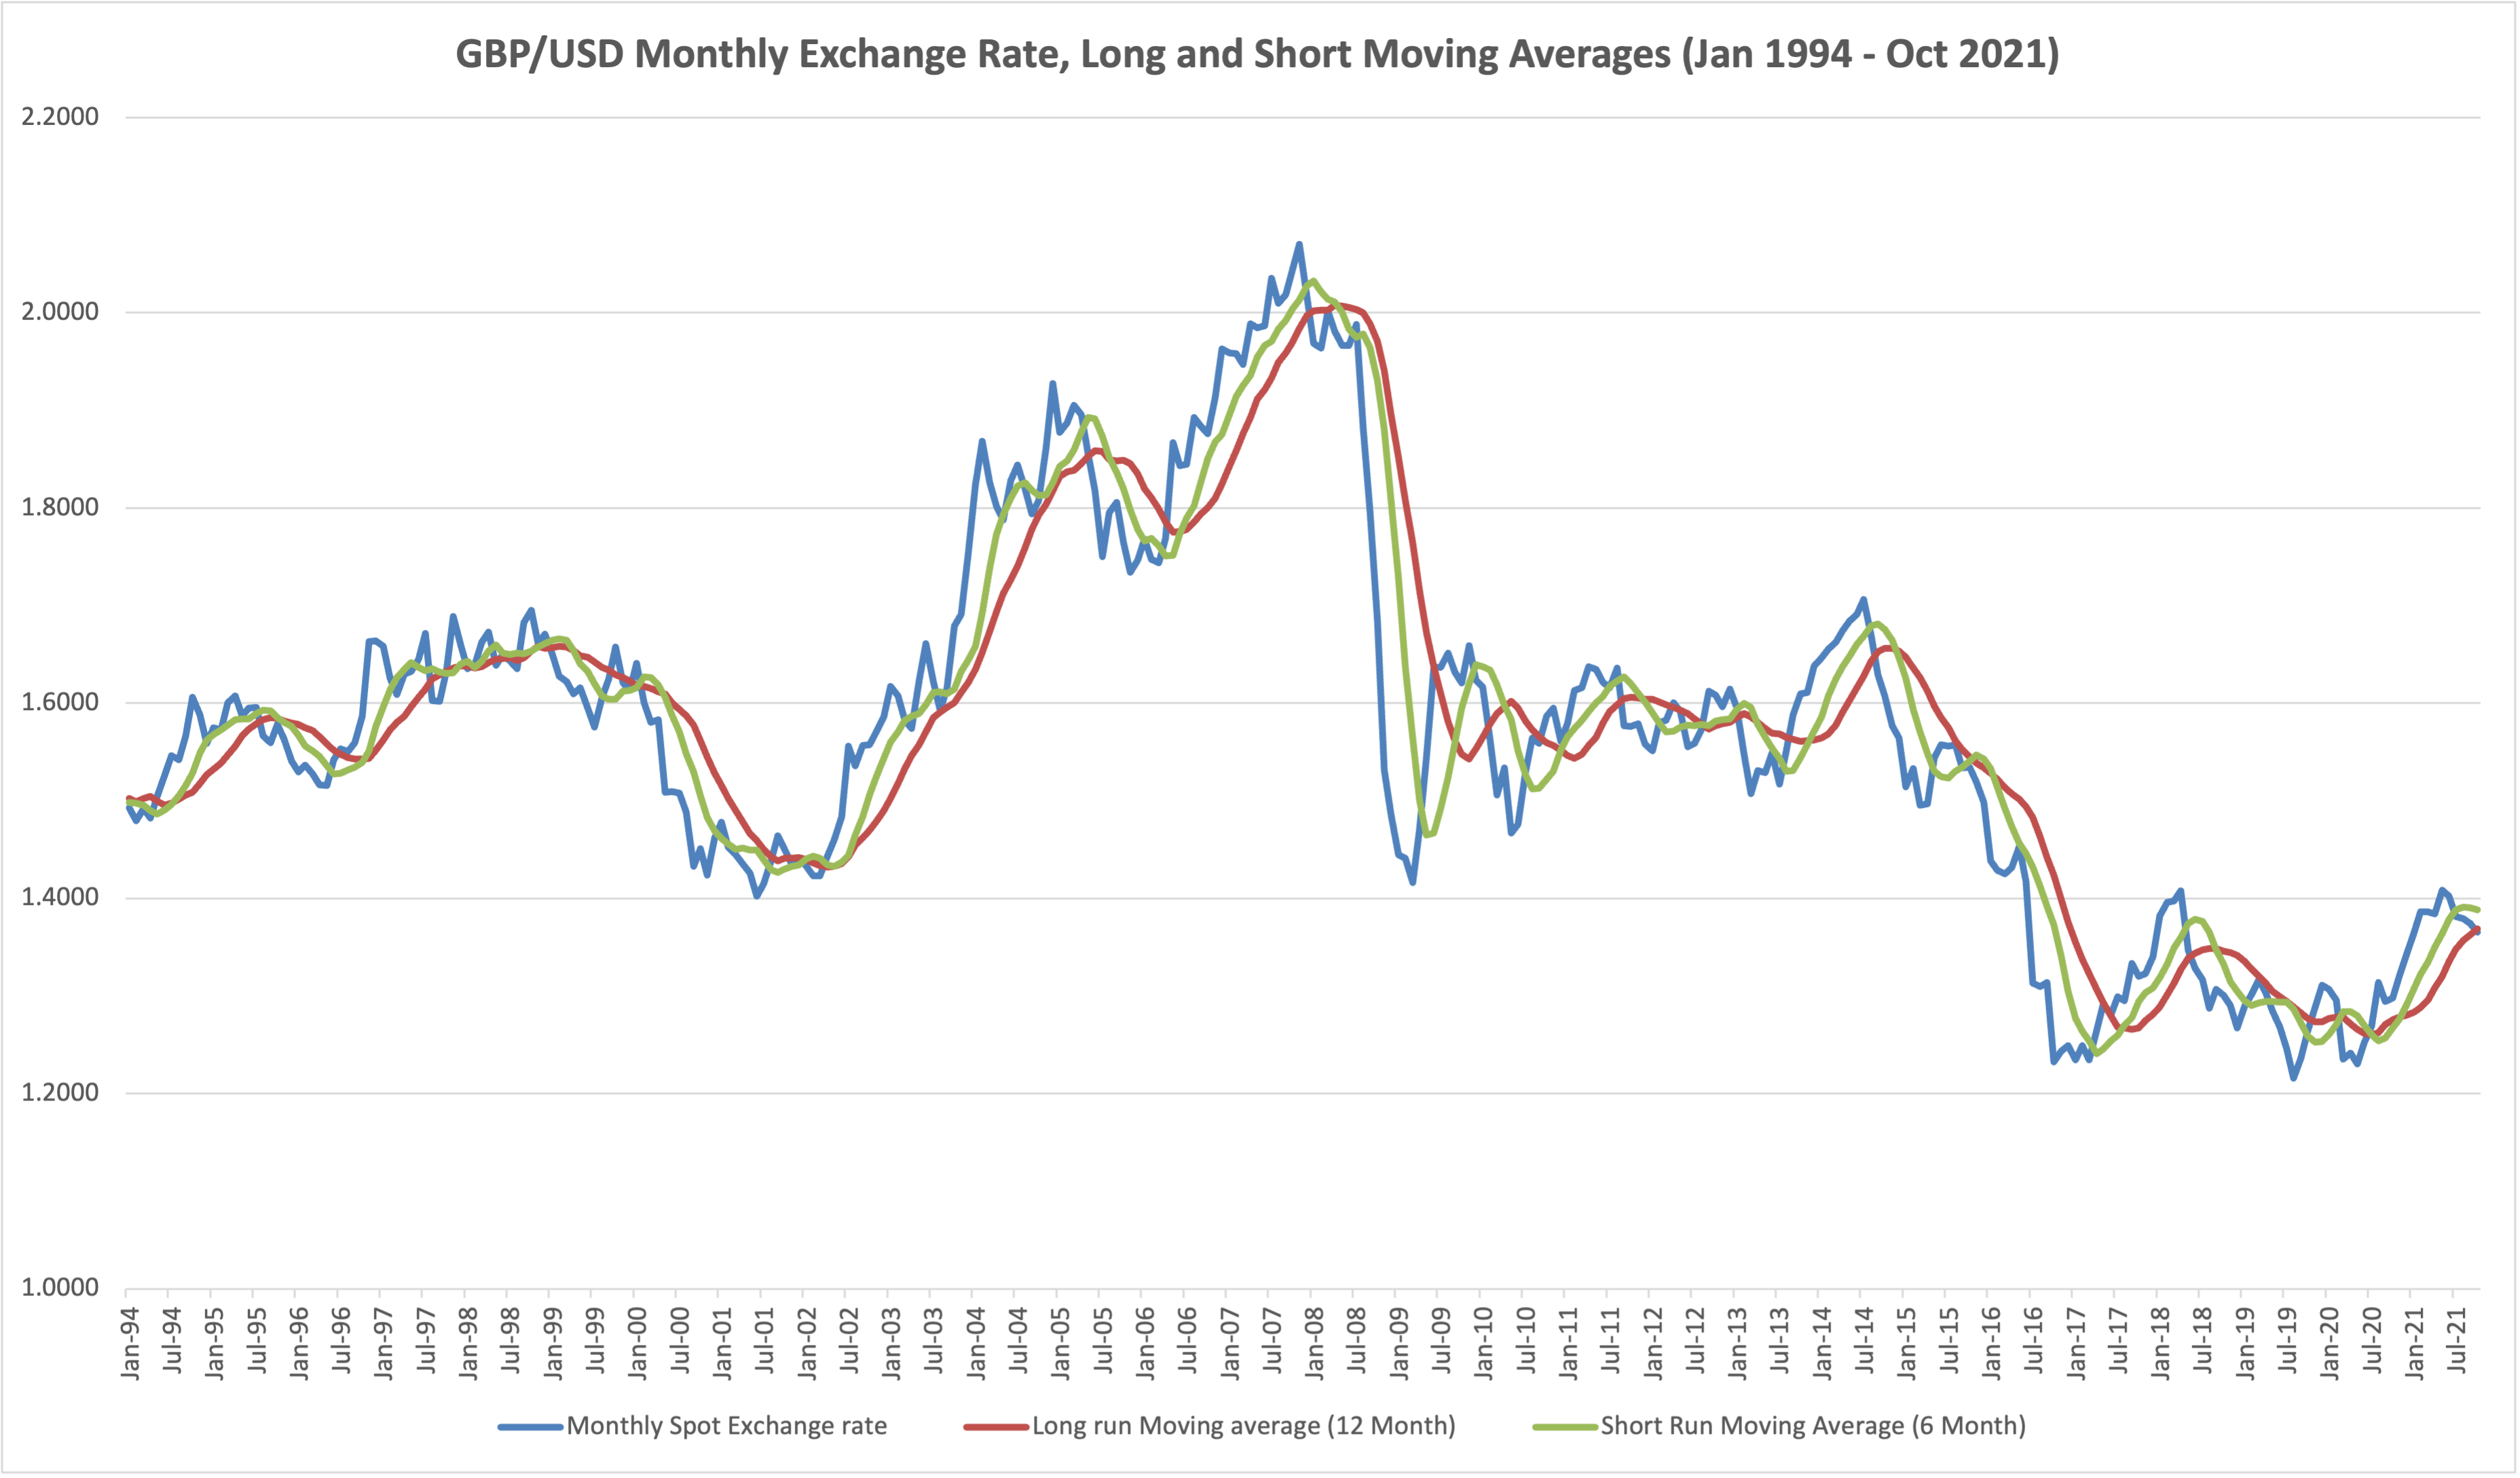
\includegraphics[width=0.75\linewidth]{GBP_USD Rates.png}
    \captionsetup{font=small, width = 0.75\linewidth}
    \caption{GBP/USD Monthly Spot Exchange rate, Long Run Moving Average $\overline{C}_{t,L}$ with $m = 12$  and Short Run Moving Average $\overline{C}_{t,S} $ with $ n = 6$}
    \label{fig:GBP/USD}
\end{figure}

Having computed long and short run averages such as the one for the GBP/USD exchange shown in figure \ref{fig:GBP/USD} for each FCU/USD pairing, we can design our momentum trading strategy. The US investor compare the a short run and long run moving averages of each exchange rate and accordingly will go long if the short run moving average is higher than the long run and will go short vice versa. This strategy assumes one can exploit short run trends in the exchange rate and that if the rate has increased recently it is likely to increase further in the near future. These trends, if they exist, arise from investors’ behavioural biases and represent a deviation from market efficiency. Our strategy can be represented algebraically as in (\ref{eq:4}).

\begin{equation}\label{eq:4}
MA(m,n) = \frac{1}{m}\sum_{i=0}^{m-1} S_{t-1} - \frac{1}{n}\sum_{i=0}^{n-1} S_{t-1}
\end{equation}
\[
\text{where  } m < n
\]

The momentum return at month $t$ for a currency position is given as the simple return if the US investor will buy the currency that month given $MA(m,n)>0$ or if the short run moving average is less than the long run moving average, $MA(m,n) < 0$, then the investor will sell the currency and earn the negative of the simple return. Since the scope of the case study prescribed investigating the trading strategy on a equally weighted portfolio of all G10 currencies we can calculate portfolio monthly returns as the average of all the individual positions. Initialising an equally weighted Portfolio with arbitrary value of 100 in December 1993, we can observe how the portfolio value changes over time. As in Figure \ref{fig:Portfolio Values} we can compare the momentum portfolio with a passively managed equal-weighted portfolio in which portfolio monthly returns is the average simple return of the currencies.  

\begin{figure}[h!]
    \centering
    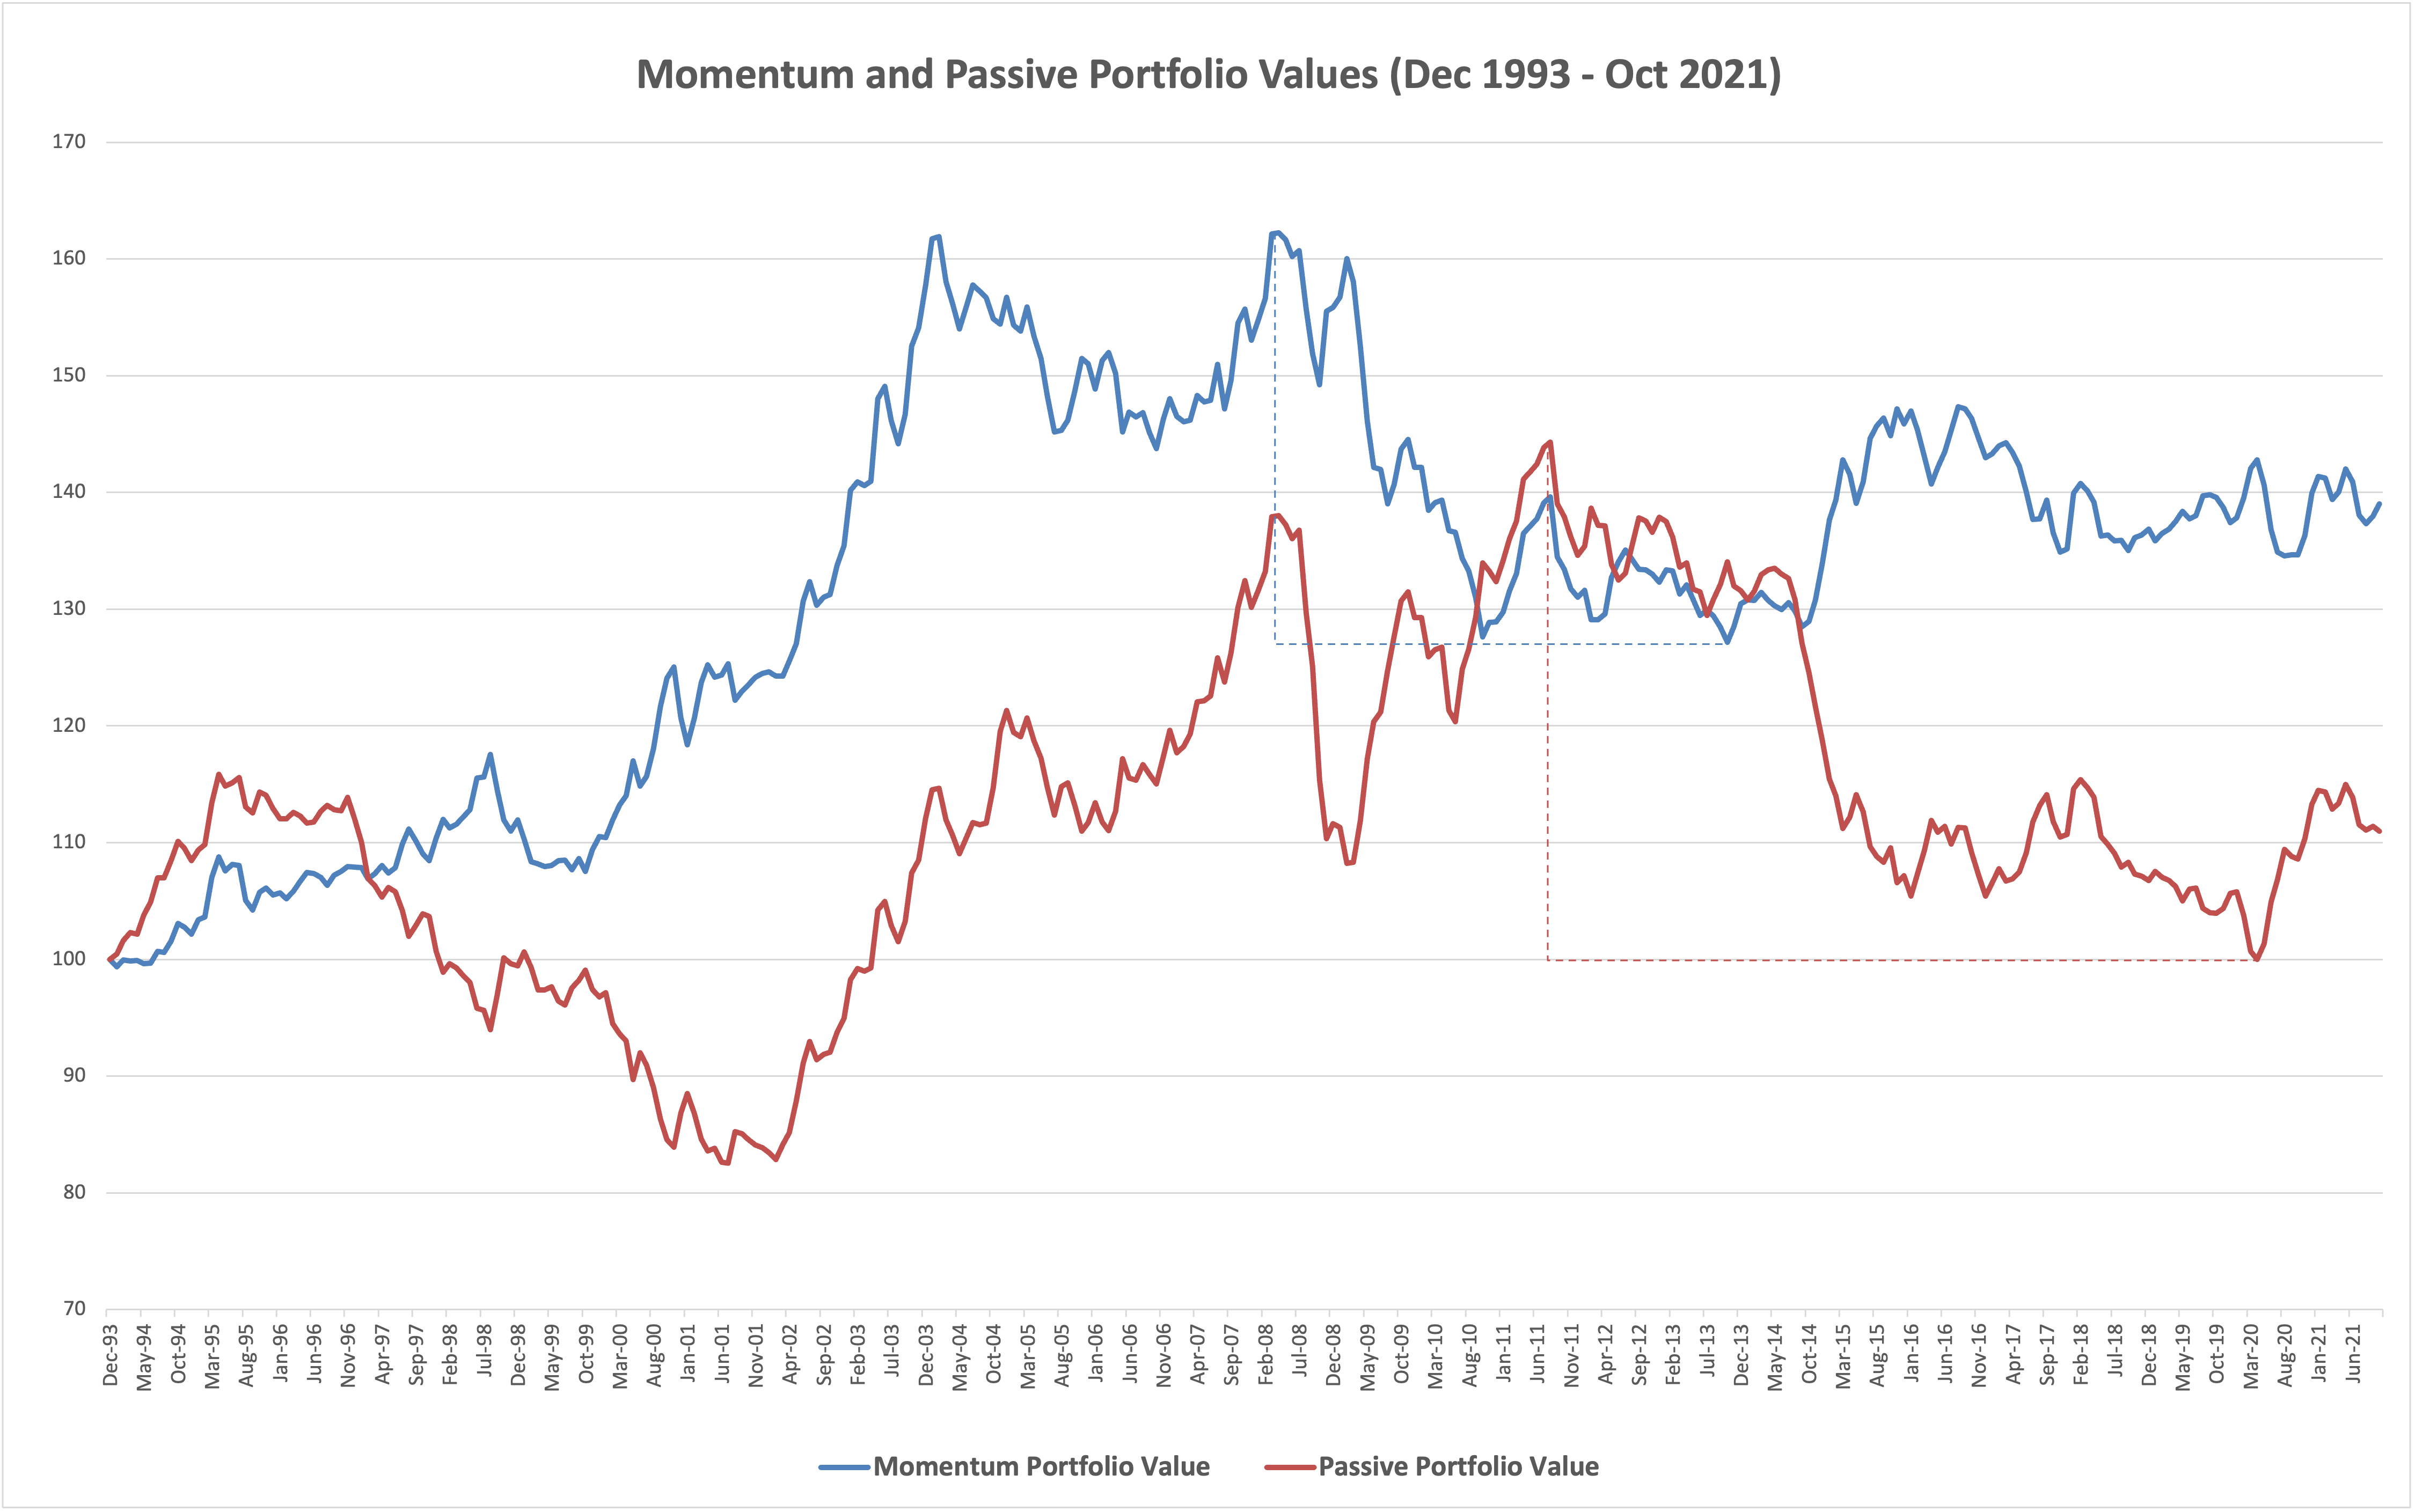
\includegraphics[width=0.75\linewidth]{Figure 2.png}
    \captionsetup{font=small, width = 0.75\linewidth}
    \caption{Momentum (m=12, n=6) traded and passively managed portfolio values over time. Maximum Drawdown for each portfolio is indicated with dashed line. }
    \label{fig:Portfolio Values}
\end{figure}

After generating portfolio values for a portfolio that is managed with a momentum strategy (m=12, n=6) and a passively managed one. We can calculate the metrics in table \ref{table:performance} to compare profitability. 

\begin{table}
    \centering
    
    \caption{Performance Metrics for Momentum and Passive Strategies}
    \label{table:performance}
    \begin{tabular}{lccc}
        \toprule
        & \textbf{Momentum} & \textbf{Passive} \\
        \midrule
        Average return & 0.11\% & 0.05\% \\
        SD & 1.41\% & 1.75\% \\
        Sharpe ratio & 0.077 & 0.027 \\
        Maximum drawdown & 21.62\% & 30.71\% \\
        \bottomrule
    \end{tabular}
\end{table}

The average monthly return for between december 1993 and octeber 2021 for the momentum portfolio is $0.11\%$ (2d.p.), and it is evident that even simple active strategies can quite easily exceed returns from a passively managed portfolio which averaged $0.05\%$ monthly returns. The standard deviation, which describes the average deviation for the portfolio returns from the expected (mean) return is lower for the momentum portfolio indicating less volatility. As a first measure of risk adjusted returns we compute the Sharpe ratio for each portfolio with equation (\ref{eq:5}). Notice that in the case study since we don't consider interest rate returns when holding foreign currencies we can assume $R_{f} = 0$, this will be elaborated further.  While more will be said about the validity of the sharpe ratios, the higher value for the momentum portfolio suggests a higher risk adjusted performance for the momentum (6,12) than the passive portfolio. The maximum drawdown, which is the largest cumulative reduction in portfolio value, $V_{t}$ over a period of time is calculated via equation (\ref{eq:6})

\begin{equation}\label{eq:5}
    S_{p}=\frac{E(R_{p})-R_{f}}{\sigma_{p}}=\frac{E(R_{p})}{\sigma_{p}}
\end{equation}

\begin{equation}\label{eq:6}
        MDD = \text{max}_{t=1,...,T}\frac{-(V_{t}-\text{max}_{i=1,...,t-1}(V_{t-i}))}{(\text{max}_{i}(V_{t-i})}
\end{equation}


\newpage\section*{How would a practitioner make use of the findings of the case study?}

\newpage\section*{What are the limitations of the modelling approaches used in the case study?}

\newpage\section*{What improvements could you make	to the	analysis if	you	had	more time or better data?}

\bibliographystyle{apalike} 
\bibliography{Bibliography.bib}

\end{document}